% =============================================================================
% Capítulo 1 — Introducción
% Base saneada desde la propuesta final y adaptada al estado real del informe
% =============================================================================

\section{Introducción}

La documentación de hardware técnico complejo ---como drones y otros sistemas electromecánicos multicomponente--- enfrenta un desafío de comunicación espacial cuando depende de imágenes 2D, planos convencionales y documentos PDF estáticos. A lo largo de este trabajo, el término \textit{hardware complejo} designa sistemas con integración estructural, energética, electrónica y de control, alta densidad de relaciones espaciales entre piezas y necesidad de inspección visual detallada del ensamblaje. Bajo estas condiciones, los medios estáticos obligan a ingenieros y técnicos a reconstruir mentalmente relaciones tridimensionales que no se presentan de forma explícita, lo que incrementa la demanda cognitiva asociada a la tarea y dificulta la lectura técnica del sistema (Sweller, 1988; Hegarty \& Waller, 2004).

Esta dificultad no es exclusiva del sector de drones. En industrias que diseñan, ensamblan, operan o mantienen hardware complejo, la geometría CAD, las listas de materiales, los manuales, la telemetría, los historiales de mantenimiento y el conocimiento experto suelen encontrarse distribuidos en sistemas separados. La literatura sobre \textit{digital twins} identifica esa fragmentación y la falta de interoperabilidad como barreras recurrentes para convertir representaciones digitales en herramientas útiles durante el ciclo de vida del producto (Jones et al., 2020; Lin et al., 2023). Por ello, antes de aspirar a un gemelo digital operacional, muchas organizaciones requieren una capa previa: un modelo visual-semántico confiable que permita comprender, inspeccionar y preparar el producto para futuras integraciones de datos (véase la Figura \ref{fig:fragmentacion_hardware_complejo}).

\begin{figure}[htbp]
    \caption{Fragmentación de información en hardware complejo.}
    \label{fig:fragmentacion_hardware_complejo}
    \centering
    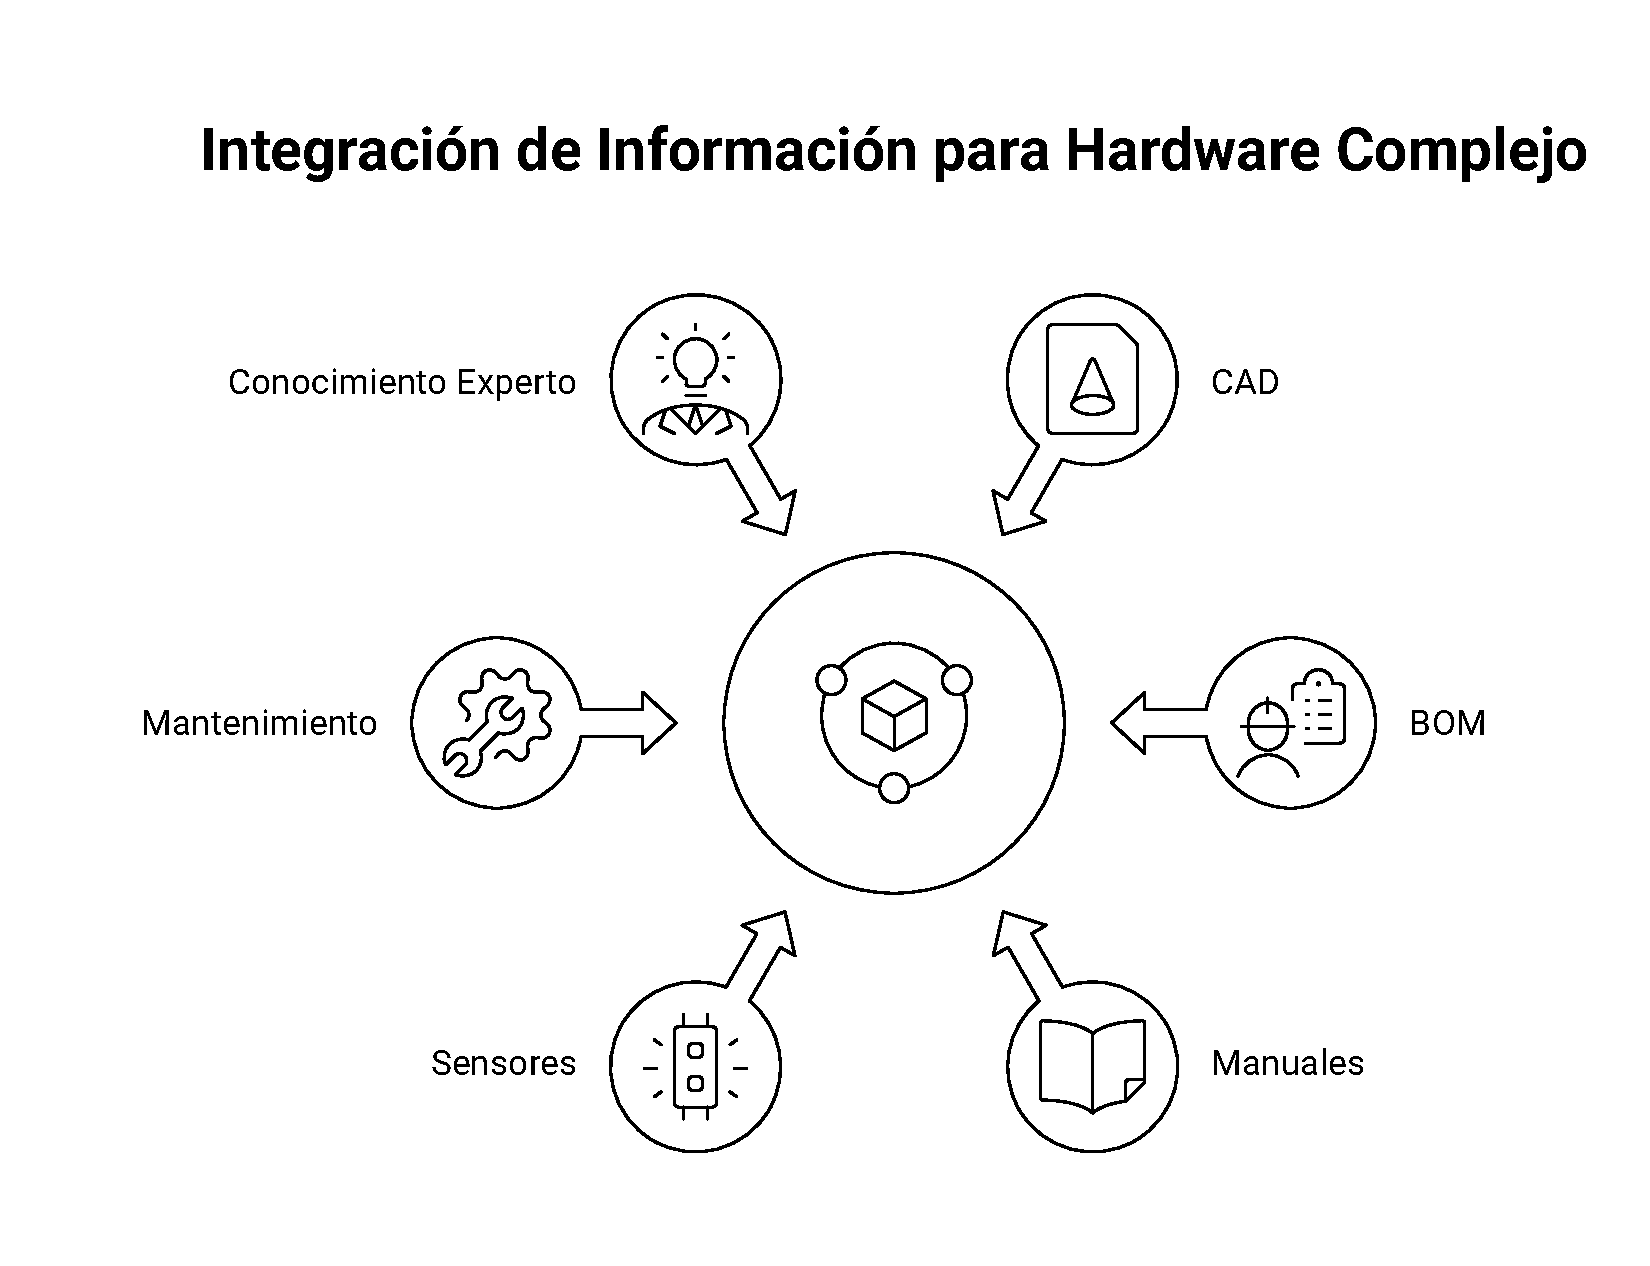
\includegraphics[width=0.88\textwidth,height=0.58\textheight,keepaspectratio]{figures/chapter1/fig_1_fragmentacion_hardware_complejo.pdf}
    \par\vspace{0.5\baselineskip}
    \apanote{El diagrama sintetiza la separación habitual entre CAD, BOM, manuales, sensores, mantenimiento y conocimiento experto como punto de partida para una capa visual-semántica. Elaboración propia.}
\end{figure}

La convergencia entre WebAssembly, WebGL y \textit{pipelines} contemporáneos de renderizado físicamente basado abrió una oportunidad concreta para trasladar parte de esa interpretación espacial al propio sistema interactivo (Yu et al., 2023). Sobre esa base, el proyecto se orientó al diseño, desarrollo y documentación de un prototipo web 3D interactivo para la visualización técnica, inspección y análisis visual del ensamblaje del dron Holybro X500~V2, buscando un equilibrio entre claridad técnica, rendimiento web y coherencia de experiencia de usuario.

\subsection{Planteamiento del problema}

La migración de documentación técnica a entornos 3D interactivos no depende solo de una mejor presentación visual. También exige resolver restricciones reales de despliegue web. Los modelos CAD de ingeniería, basados en NURBS, ensamblajes extensos y activos de alta densidad geométrica, no son directamente compatibles con las condiciones de ejecución de una aplicación web. Si bien WebAssembly permite el crecimiento dinámico de la memoria lineal, la viabilidad práctica del producto depende de dos factores: controlar la huella inicial de los activos y configurar un \textit{heap} contiguo lo suficientemente grande para sostener datos, geometría y ejecución estable en el navegador (Unity Technologies, 2024a; WebAssembly Community Group, s.\,f.).

En este proyecto, el problema técnico se articuló en cuatro dimensiones complementarias (véase la Figura \ref{fig:nucleo_problemico_dimensiones}):

\begin{itemize}
    \item \textbf{Huella inicial de datos.} Los modelos CAD originales pueden alcanzar decenas o cientos de megabytes, e incluso más en ensamblajes extensos, por lo que requieren limpieza, simplificación geométrica, \textit{baking} y empaquetado selectivo para ser viables en web.
    \item \textbf{Rendimiento en tiempo real.} Mantener 30 FPS o más, equivalente a un \textit{frame time} de aproximadamente 33,33\,ms, exige controlar presupuesto geométrico, materiales, \textit{draw calls} y estados de render.
    \item \textbf{Latencia de interacción.} Alternativas como \textit{Pixel Streaming} pueden ofrecer render remoto de alta calidad visual, pero introducen dependencia de infraestructura, red y latencias poco adecuadas para inspección técnica precisa (Epic Games, s.\,f.-a, s.\,f.-b).
    \item \textbf{Fragmentación de datos técnicos.} La geometría del producto no basta para explicar su función, mantenimiento o evolución. Para que una representación digital avance hacia \textit{digital shadow} o \textit{digital twin}, debe existir una relación trazable entre piezas, metadatos, procedimientos, sensores, eventos y decisiones de soporte (Kritzinger et al., 2018; Digital Twin Consortium, 2020).
\end{itemize}

\begin{figure}[htbp]
    \caption{Dimensiones del núcleo problemático del proyecto.}
    \label{fig:nucleo_problemico_dimensiones}
    \centering
    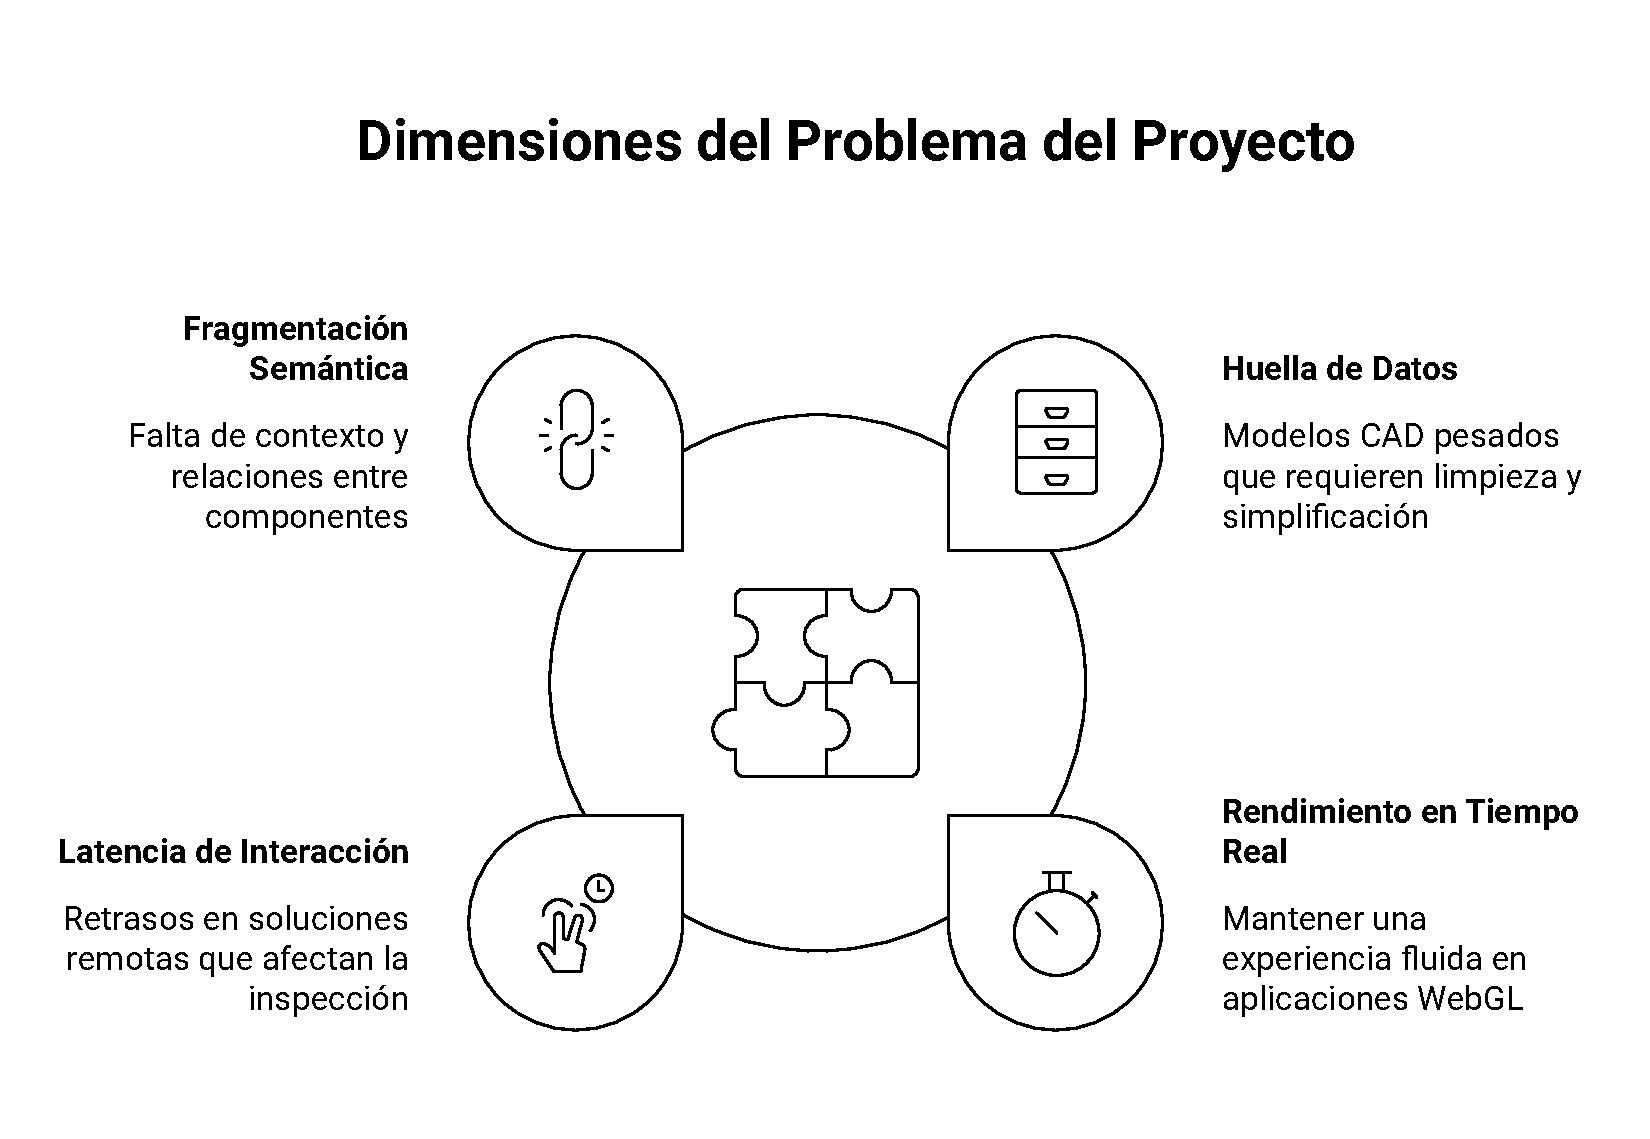
\includegraphics[width=0.92\textwidth,height=0.58\textheight,keepaspectratio]{figures/chapter1/fig_1_nucleo_problematico_dimensiones.pdf}
    \par\vspace{0.5\baselineskip}
    \apanote{La figura resume los cuatro frentes que condicionan la viabilidad del prototipo: huella inicial de datos, rendimiento en tiempo real, latencia de interacción y fragmentación semántica. Elaboración propia.}
\end{figure}

Se identificó, por tanto, la necesidad de documentar un \textit{pipeline} de \textit{Technical Art} que permitiera desplegar hardware complejo en un visor 3D web con orientación espacial suficiente para tareas de inspección, costo computacional controlado y capacidad de análisis visual del ensamblaje para propósitos académicos e ingenieriles.

El proyecto se orientó por dos preguntas de investigación complementarias:

\begin{enumerate}
    \item \textbf{¿Qué diferencias descriptivas se observan en el desempeño de tareas y la carga de trabajo percibida cuando usuarios con perfil afín realizan actividades de exploración e identificación del dron Holybro X500~V2 mediante un prototipo web 3D interactivo, en comparación con un soporte 2D de referencia? Adicionalmente, ¿bajo qué condiciones de rendimiento y memoria resulta técnicamente viable dicho prototipo en el navegador?}
    \item \textbf{¿Cuál es el nivel de usabilidad percibida del prototipo 3D medido con SUS tras su uso?}
\end{enumerate}

\subsection{Justificación}

La elección de Unity Web frente a bibliotecas nativas de JavaScript o soluciones de \textit{streaming} remoto no obedeció a un menor tamaño de \textit{build}. La decisión se sustentó en la integración del \textit{pipeline}, la capacidad de extensión técnica, el soporte para materiales y shaders, y la posibilidad de mantener un flujo coherente entre programación, arte técnico y evaluación del prototipo.

Desde la perspectiva industrial, el valor del proyecto radica en cerrar una primera brecha de madurez digital: transformar un producto electromecánico multicomponente en una experiencia web navegable, seleccionable, explicable y medible. En este sentido, el prototipo funciona como un \textit{visual product twin} o \textit{technical product twin}: una capa visual-semántica que todavía no sincroniza telemetría real, pero sí prepara identificadores, jerarquías, categorías, fichas y herramientas de inspección que podrían alimentar fases posteriores de \textit{digital shadow} y \textit{digital twin} operacional (Kritzinger et al., 2018; Digital Twin Consortium, 2020; Lin et al., 2023; véase la Figura \ref{fig:alcance_visual_product_twin}).

\begin{figure}[htbp]
    \caption{Alcance actual del proyecto frente a un gemelo digital operacional.}
    \label{fig:alcance_visual_product_twin}
    \centering
    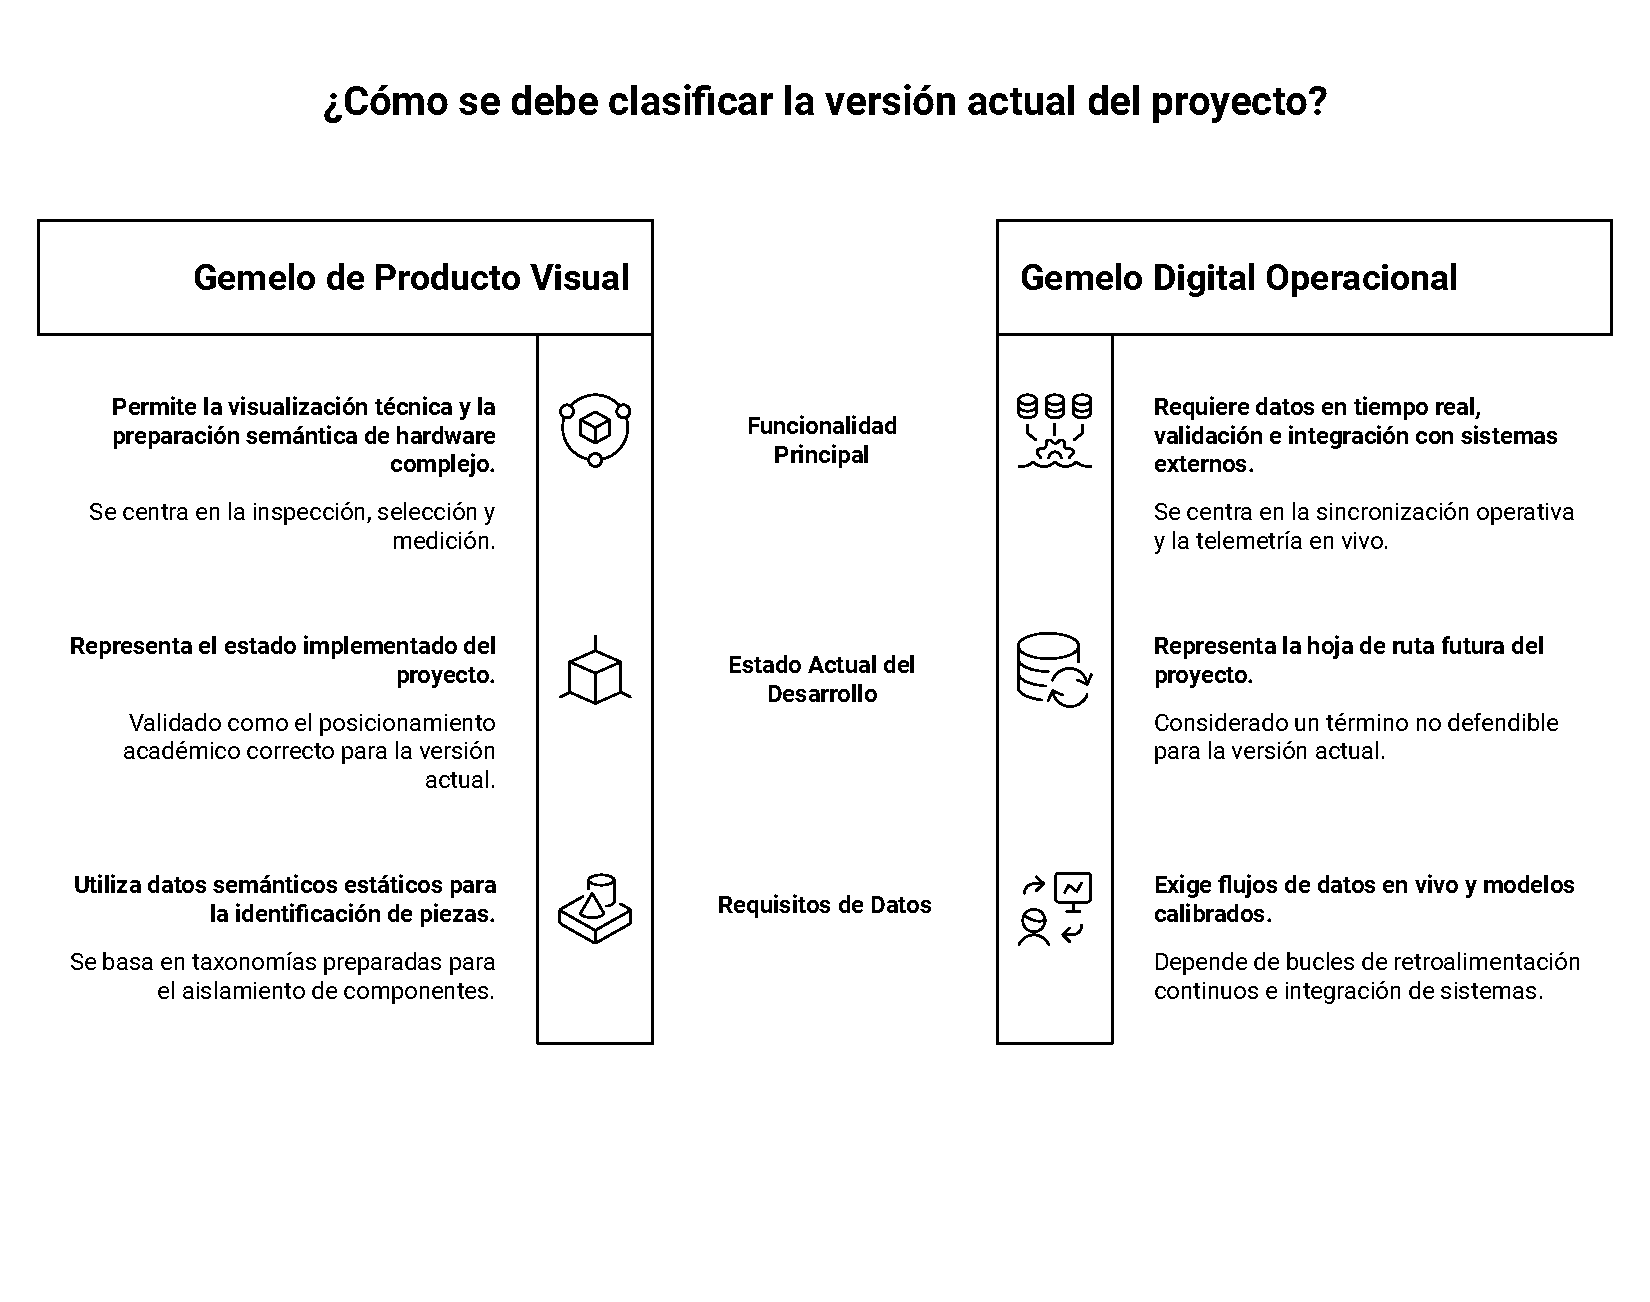
\includegraphics[width=\textwidth,height=0.66\textheight,keepaspectratio]{figures/chapter1/fig_1_alcance_visual_product_twin.pdf}
    \par\vspace{0.5\baselineskip}
    \apanote{La versión final se posiciona como \textit{visual product twin}: integra inspección, selección y preparación semántica, pero no telemetría real, sincronización operacional ni modelos calibrados. Elaboración propia.}
\end{figure}

\subsubsection{Trade-off explícito entre tooling y huella inicial}

Unity no fue seleccionado por ofrecer la descarga inicial más ligera. Por el contrario, el proyecto aceptó una huella inicial mayor a cambio de un ecosistema de autoría más consistente: editor integrado, \textit{profiling}, flujo de materiales, UI Toolkit, sistema de escenas y facilidad para extender el comportamiento mediante C\# y shaders personalizados (Unity Technologies, 2024b, 2024d).

\subsubsection{Ejecución de lógica compilada en WebAssembly}

En el target web, Unity convierte código intermedio de .NET a C++ mediante IL2CPP y posteriormente compila ese resultado a WebAssembly usando el \textit{toolchain} del \textit{build}. Esto permitió sostener una base tipada para la lógica interactiva del prototipo y mantener el proyecto dentro de un entorno técnico unificado, sin atribuir a IL2CPP, por sí solo, todo el salto a Wasm (Unity Technologies, 2024c; Unity Technologies, s.\,f.).

\subsubsection{\textit{Pipeline} integrado de importación y renderizado}

El proyecto exigía coordinar limpieza de activos CAD, materiales PBR, UI responsiva, modos analíticos y validación funcional sin fragmentar el flujo entre demasiadas herramientas. Unity aportó un entorno integrado para importar geometría, gestionar materiales, perfilar rendimiento y desplegar un \textit{build} web desde una misma base de trabajo.

\subsubsection{Capacidad de extensión para visualización técnica}

La aplicación final no se concibió como un visor pasivo de un modelo tridimensional, sino como una experiencia de inspección técnica. El usuario puede recorrer el ensamblaje, seleccionar componentes, aislar zonas de interés, consultar información contextual, separar visualmente el conjunto para comprender relaciones de montaje, observar cortes del interior y alternar lecturas visuales que resaltan materialidad, estructura o comportamiento térmico aproximado. Estas capacidades exigían una plataforma capaz de articular renderizado realista, interacción con piezas, organización semántica del hardware y herramientas de análisis visual dentro de un mismo producto.

\subsubsection{Compatibilidad esperada de la plataforma web}

La plataforma web de Unity contempla navegadores compatibles de escritorio y algunos navegadores móviles, aunque el comportamiento efectivo depende del navegador, su versión, la memoria disponible y el nivel de optimización del \textit{build} (Unity Technologies, s.\,f.). Por ello, en este trabajo la compatibilidad móvil se documenta como \textit{compatibilidad esperada}, sin pretender constituir una garantía universal ni una validación exhaustiva sobre una matriz cerrada de dispositivos.

\subsubsection{Aporte a la Ingeniería Multimedia}

El proyecto aporta al programa por al menos cuatro vías:

\begin{itemize}
    \item documenta un \textit{pipeline} técnico para llevar activos CAD a un visor web interactivo;
    \item articula computación gráfica, experiencia de usuario, documentación técnica y arte técnico en un mismo caso aplicado;
    \item convierte restricciones de rendimiento web en criterios medibles de diseño y optimización;
    \item consolida un caso de estudio pertinente para la Ingeniería Multimedia, donde la claridad técnica del ensamblaje es tan importante como la calidad visual del resultado.
\end{itemize}

\subsection{Objetivos}

\subsubsection{Objetivo general}

Desarrollar un prototipo de visualización web 3D interactiva basado en Unity Web, enfocado en la exploración técnica, la inspección y el análisis visual del ensamblaje de hardware complejo, optimizado mediante criterios de \textit{Technical Art} para su despliegue eficiente en navegadores web compatibles.

\subsubsection{Objetivos específicos}

\begin{enumerate}
    \item Diseñar un \textit{pipeline} de optimización de activos 3D que reduzca la carga poligonal de modelos CAD originales hasta un presupuesto geométrico compatible con WebGL, preservando la legibilidad formal del ensamblaje, la identificación correcta de piezas y la lectura espacial suficiente para inspección técnica mediante retopología, limpieza de mallas y \textit{baking} de texturas.
    \item Integrar en Unity URP un sistema de materiales y modos de visualización que combine renderizado realista con herramientas de inspección técnica, procurando un \textit{frame time} igual o inferior a 33,33\,ms (30 FPS o más) bajo el entorno de prueba controlado definido para la validación del \textit{build} web.
    \item Implementar el prototipo interactivo en la plataforma web de Unity con lógica desarrollada en C\# y desplegada mediante la cadena de compilación del motor ---conversión de ensamblados administrados, generación intermedia de C++ y ejecución en WebAssembly---, de modo que habilite navegación orbital, selección de piezas, consulta contextual de información y herramientas como vista explosionada, corte transversal y modos analíticos.
    \item Evaluar de manera formativa el desempeño en tareas y la carga de trabajo percibida por condición (3D vs.\ 2D) mediante pruebas con usuarios, NASA-TLX Raw y protocolo \textit{Think-Aloud}, y estimar adicionalmente la usabilidad percibida del prototipo 3D mediante SUS tras su uso; todo ello contrastado de forma descriptiva y frente a las metas operativas definidas para el proyecto.
\end{enumerate}

\subsection{Alcance y limitaciones}

El alcance del presente trabajo se circunscribió al desarrollo de un \textbf{Producto Mínimo Viable} (MVP) técnico y académico orientado a documentar la viabilidad de un visor web 3D interactivo para hardware complejo. El caso de estudio seleccionado fue el dron Holybro X500~V2 porque cuenta con recursos técnicos de libre acceso, archivos CAD/STEP consultables, documentación pública y abundantes referencias abiertas en internet. Esta disponibilidad permitió ejecutar el proyecto sin depender de material propietario restringido, sin comprometer derechos de autor y con suficiente trazabilidad para justificar decisiones de modelado, documentación e interpretación técnica.

Las principales delimitaciones fueron las siguientes:

\begin{itemize}
    \item \textbf{Modelo único.} El prototipo se desarrolló sobre un único modelo de referencia, aunque la arquitectura quedó preparada para generalizar catálogos, datos y saneamiento de runtime.
    \item \textbf{No constituye un digital twin operacional.} La versión final no recibe telemetría real, no sincroniza estado con un activo físico, no ejecuta diagnóstico de mantenimiento ni se integra con sistemas PLM, ERP, CMMS, SCADA o IoT. Su alcance correcto es el de una plataforma visual-semántica preparada para evolucionar hacia esas capas.
    \item \textbf{Plataforma web.} El producto se concentró en la plataforma web compilada con WebAssembly. No se desarrollaron \textit{builds} nativas independientes de escritorio o móvil.
    \item \textbf{Compatibilidad móvil acotada.} El producto se concibió para navegadores compatibles de escritorio y móviles. En el cierre de desarrollo se verificó su funcionamiento en escritorio y en dispositivos móviles reales, incluyendo teléfonos de gama media-baja como Redmi Note 10S. La compatibilidad se interpreta dentro de las condiciones de prueba de cada dispositivo, navegador, resolución y escenario, sin asumir cobertura universal sobre todo el ecosistema móvil.
    \item \textbf{Muestra de validación.} Se estableció como meta deseable un grupo de 30 participantes y como escenario mínimo operativo una muestra de entre 8 y 12 para evaluación formativa. El informe integra datos de 12 participantes anonimizados, con SUS, NASA-TLX Raw, tareas completadas y registro \textit{Think-Aloud}; por tanto, los resultados se interpretan de manera descriptiva y exploratoria, sin pretensión de inferencia estadística poblacional.
    \item \textbf{Adaptación de escritorio.} El diseño UX/UI se desarrolló con enfoque \textit{mobile-first}. La versión de escritorio es funcional y permite demostrar el prototipo, pero corresponde a una adaptación temporal del sistema móvil. Por limitaciones de tiempo no se diseñó una experiencia específica para la comodidad del usuario en PC, por lo que su ergonomía no debe interpretarse como un sistema \textit{desktop} optimizado.
    \item \textbf{Cables, conexiones y electrónica detallada.} El prototipo no incluye la totalidad de cables, conectores, arneses ni elementos electrónicos internos del dron. Integrar esa capa habría requerido modelado adicional, revisión de rutas de conexión y desarrollo de interacciones específicas dentro de Unity para consultar o aislar dichas conexiones. Por restricciones de tiempo, el alcance se concentró en la estructura principal, componentes representativos y herramientas de inspección visual.
    \item \textbf{Herramientas ocultas o no integradas.} Algunas capacidades permanecen en código, pero no forman parte de la UI final visible ni del flujo funcional documentado como estado final del producto.
\end{itemize}

\newpage
